\chapter*{CAPÍTULO VII: RELACIÓN DE PLANOS Y DISEÑO CATASTRAL}
\addcontentsline{toc}{chapter}{CAPÍTULO VII: RELACIÓN DE PLANOS Y DISEÑO CATASTRAL}

\section{CATÁLOGO OFICIAL DE PLANOS DE INGENIERÍA}

El proyecto cuenta con un conjunto integral de láminas técnicas elaboradas en formato normalizado DWG/DXF georreferenciadas en el sistema WGS 84 / UTM Zona 19 Sur:

\begin{table}[H]
\centering
\small
\begin{tabular}{|c|l|c|c|}
\hline
\textbf{Código} & \textbf{Título del Plano} & \textbf{Escala} & \textbf{Formato} \\
\hline
\textbf{PL-01} & Plano Clave General: Redes MT, SEDs y Catastro Urbano & 1:2,500 & A1 \\
\textbf{PL-02} & Trazo y Perfil Longitudinal de Línea Primaria 10 kV & H: 1:2000, V: 1:200 & A1 \\
\textbf{PL-03} & Detalle Electromecánico de Subestaciones Aéreas Biposte (SAB) & 1:50 / 1:25 & A1 \\
\textbf{PL-04} & Red de Distribución Secundaria 380/220 V y Alumbrado Público & 1:1,000 & A1 \\
\textbf{PL-05} & Detalles Típicos de Armados BT, Puestas a Tierra y Acometidas & Indicadas & A1 \\
\hline
\end{tabular}
\caption{Relación oficial de planos del expediente técnico.}
\end{table}

\section{INTEGRACIÓN CATASTRAL Y VISTAS ESPACIALES DEL PROYECTO}

A continuación se presentan las visualizaciones cartográficas y modelos vectoriales del casco urbano de Limbani empleados como base física inalterable para el replanteo y ubicación de las redes:

\subsection{Vista Satelital General con Catastro Superpuesto}
La Figura~\ref{fig:ortofoto} muestra la totalidad del casco urbano encajonado en el valle del Río Limbani, con la delimitación exacta de las 87 manzanas, 623 lotes y la traza de las vías principales y secundarias:

\begin{figure}[H]
\centering
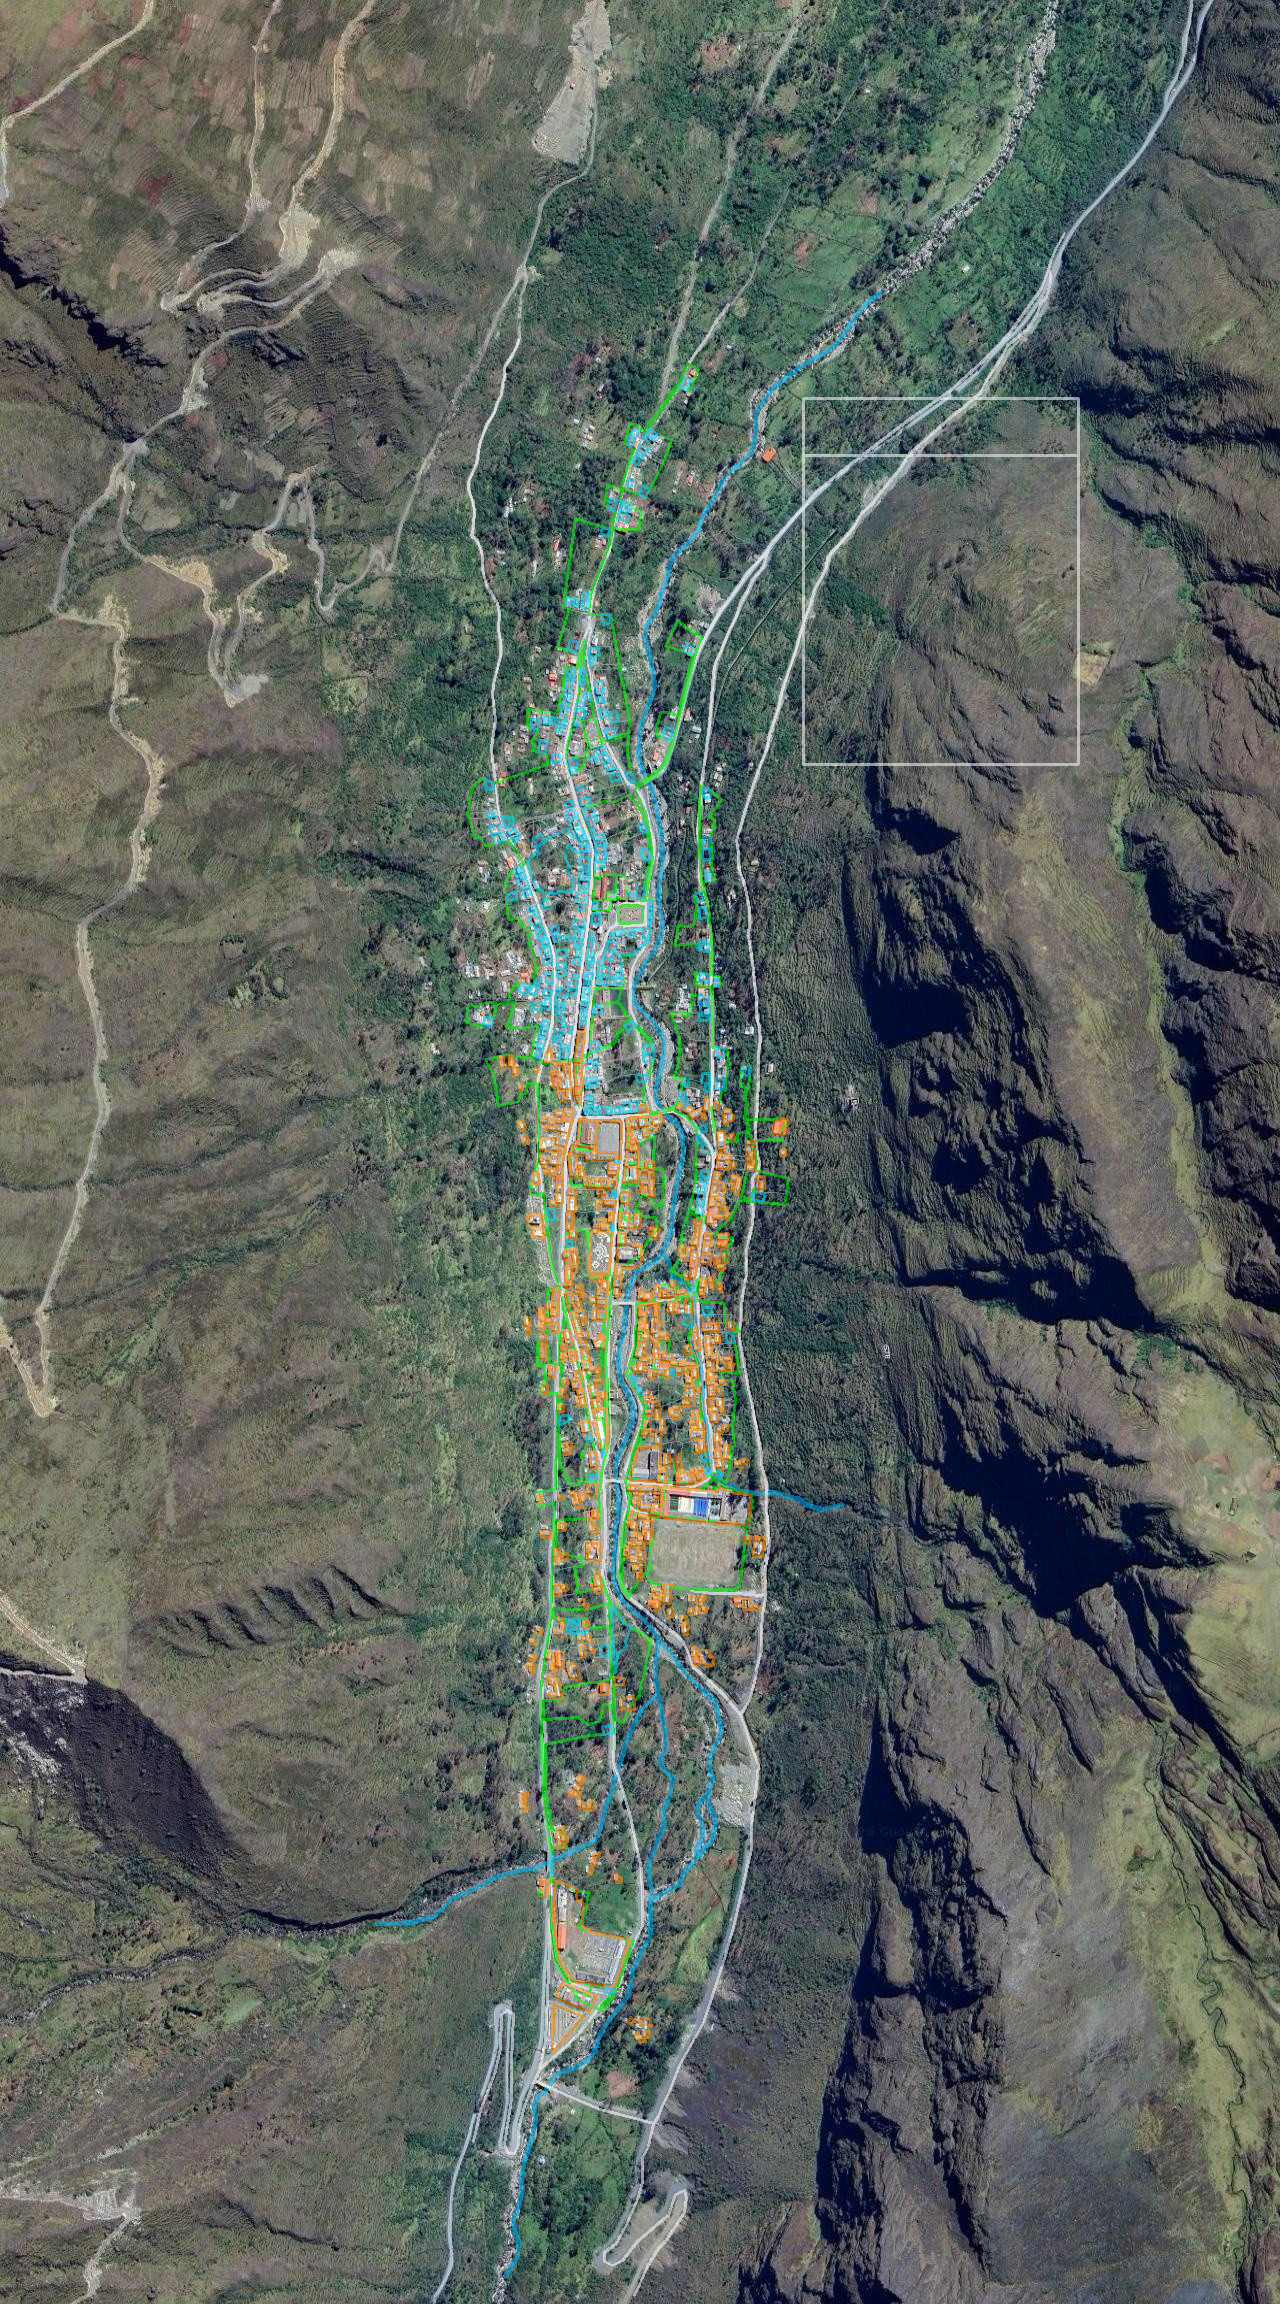
\includegraphics[width=0.85\textwidth,height=0.36\textheight,keepaspectratio]{figuras/01_superposicion_ortofoto_completa.png}
\caption{Superposición ortofotogramétrica y delimitación de manzanas catastrales en Limbani.}
\label{fig:ortofoto}
\end{figure}

\subsection{Modelo Digital Vectorial CAD del Sistema Urbano}
En la Figura~\ref{fig:cad_modelo} se observa la estructura de redes vectoriales que integra las cotas altimétricas, paramentos de predios, alineamientos de vías y cauces fluviales:

\begin{figure}[H]
\centering
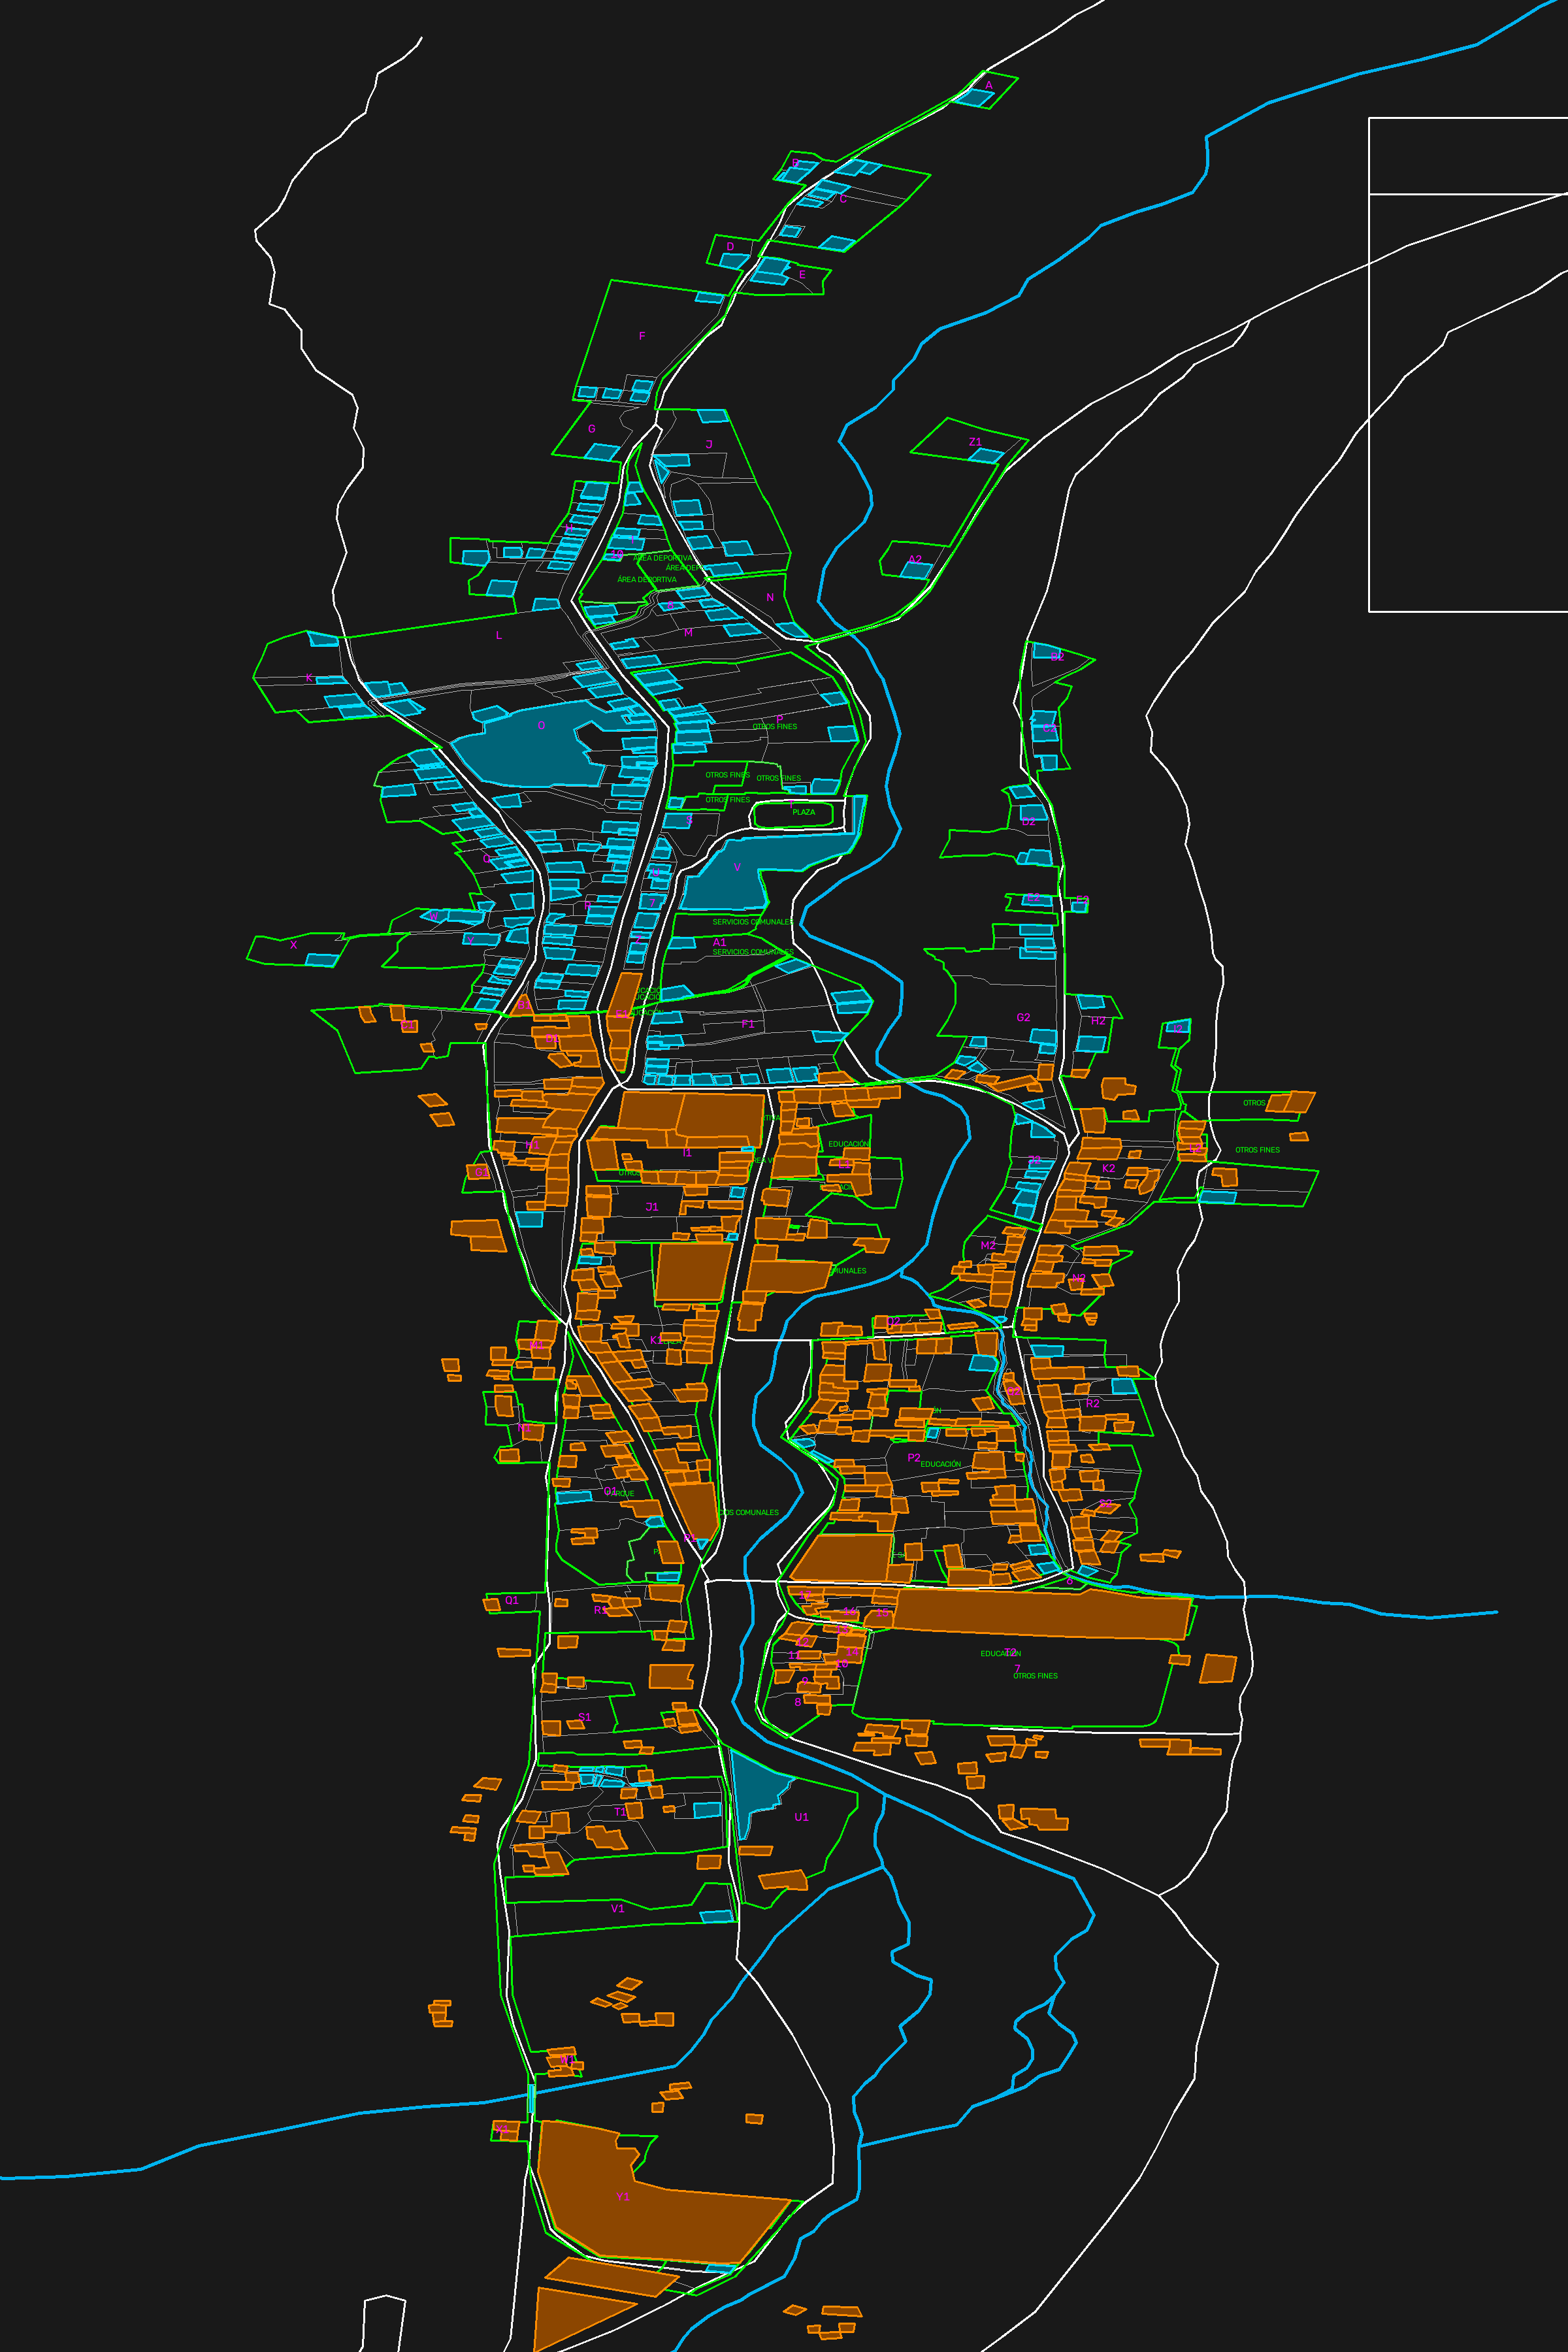
\includegraphics[width=0.85\textwidth,height=0.36\textheight,keepaspectratio]{figuras/02_modelo_autocad_completo.png}
\caption{Modelo geométrico y base catastral vectorial en formato CAD/DXF.}
\label{fig:cad_modelo}
\end{figure}

\newpage
\subsection{Plano General de Redes Eléctricas, Postería y Subestaciones}
La Figura~\ref{fig:redes_detalladas} presenta el diseño electromecánico integrado sobre el catastro oficial de Limbani, mostrando la traza de la línea de 10 kV (rojo), los 24 apoyos de media tensión, las 3 Subestaciones Biposte SED-01, SED-02 y SED-03 (bloques dorados), las retenidas de anclaje (magenta) y los 360 postes de baja tensión (azul) con las 165 luminarias de alumbrado público LED (amarillo):

\begin{figure}[H]
\centering
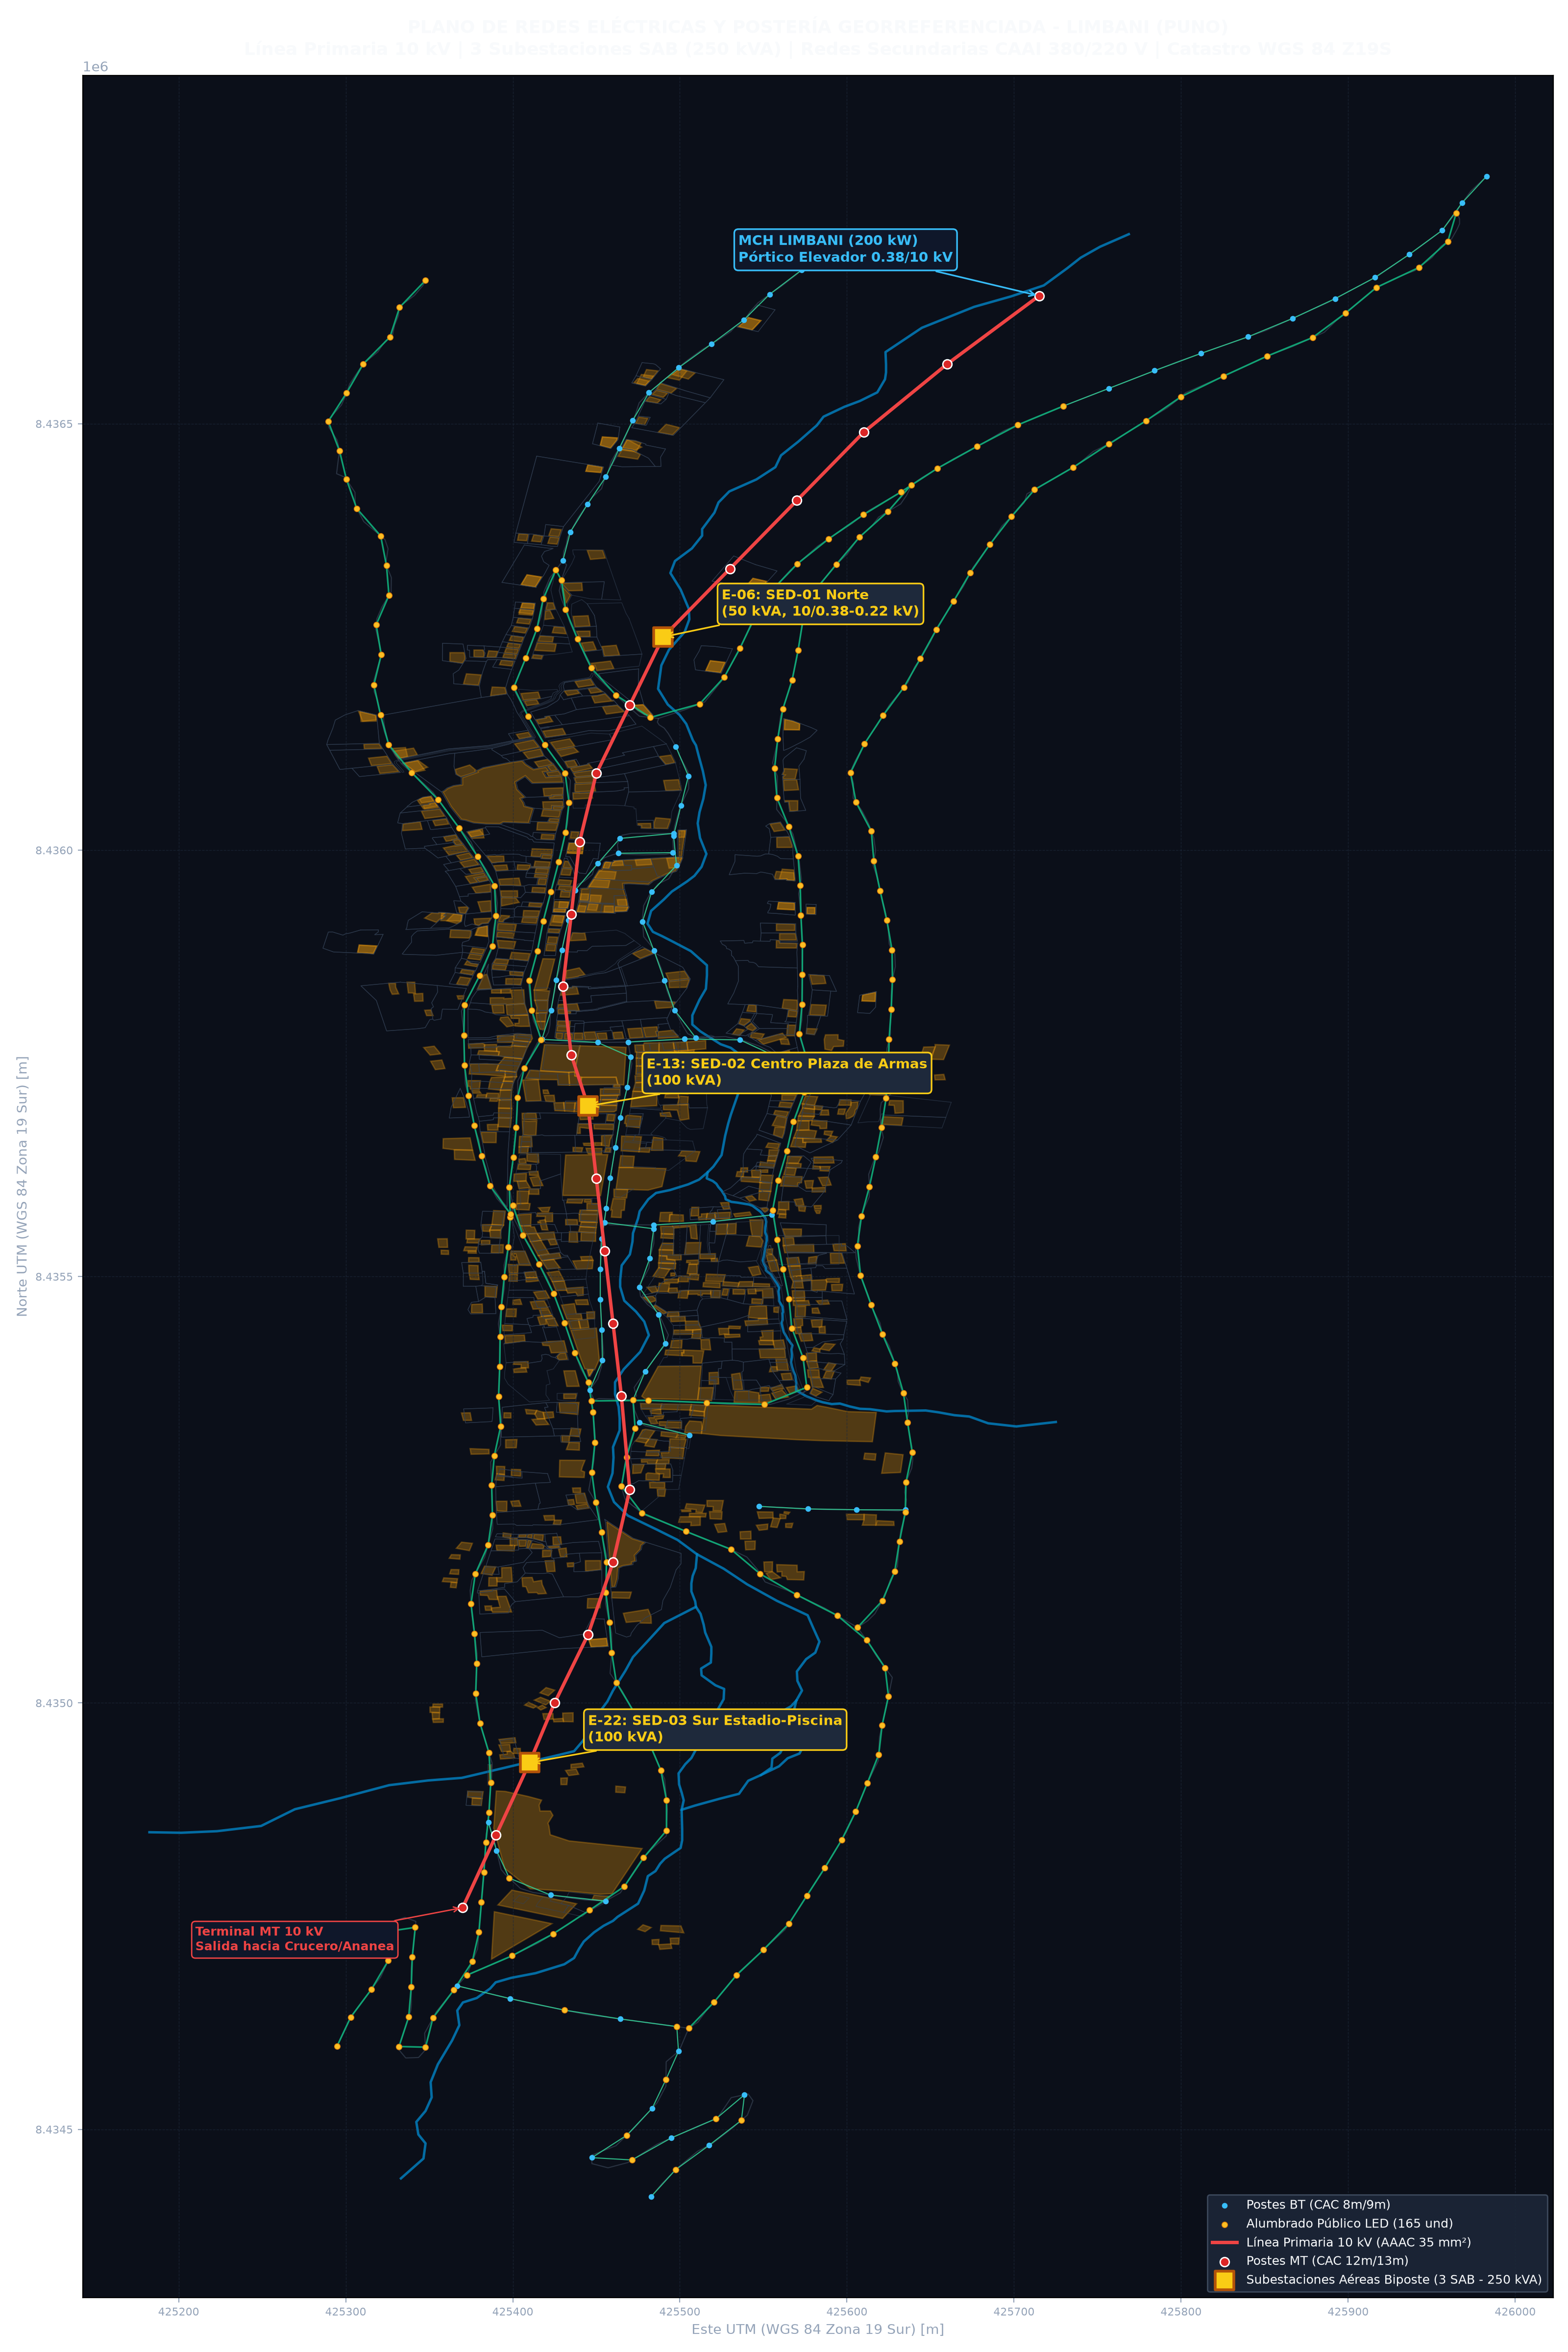
\includegraphics[width=0.85\textwidth,height=0.60\textheight,keepaspectratio]{figuras/07_redes_electricas_detalladas_catastro.png}
\caption{Plano General de Redes Eléctricas, Postería CAC y Subestaciones Aéreas Biposte georreferenciadas en Limbani (WGS 84 Z19S).}
\label{fig:redes_detalladas}
\end{figure}

\newpage
\subsection{Detalle Sector Norte: Casa de Máquinas MCH Limbani y SED-01}
La Figura~\ref{fig:sector_norte} muestra la zona de captación y casa de máquinas de la Minicentral Hidroeléctrica (200 kW con turbina Michell-Banki), el pórtico de salida en 10 kV y la alimentación a la Subestación SED-01 (Norte, 50 kVA) que abastece a 142 lotes:

\begin{figure}[H]
\centering
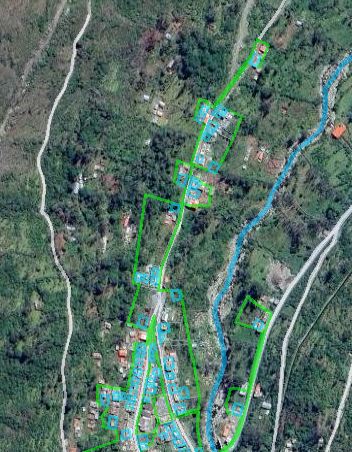
\includegraphics[width=0.85\textwidth,height=0.36\textheight,keepaspectratio]{figuras/03_zoom_sector_norte_hidroelectrica.png}
\caption{Sector Norte: Casa de máquinas MCH Limbani y cobertura de SED-01.}
\label{fig:sector_norte}
\end{figure}

\subsection{Detalle Sector Centro: Plaza de Armas y SED-02}
La Figura~\ref{fig:sector_centro} exhibe el núcleo cívico y comercial de Limbani, donde se emplaza la SED-02 (Centro, 100 kVA) que energiza la Plaza de Armas, Municipalidad, Centro de Salud y 348 lotes de alta densidad:

\begin{figure}[H]
\centering
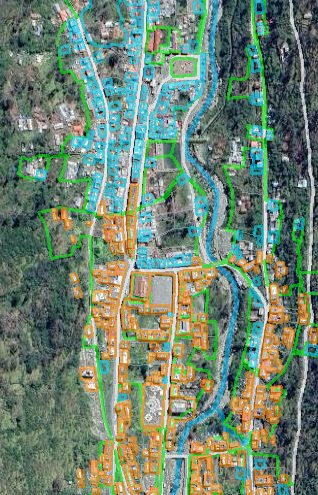
\includegraphics[width=0.85\textwidth,height=0.36\textheight,keepaspectratio]{figuras/04_zoom_sector_centro_plaza_puno.png}
\caption{Sector Centro: Plaza de Armas de Limbani y cobertura de SED-02.}
\label{fig:sector_centro}
\end{figure}

\newpage
\subsection{Detalle Sector Confluencia Fluvial y Estadio Municipal}
La Figura~\ref{fig:sector_confluencia} ilustra la confluencia entre el Río Limbani y la Quebrada Chinchalamani, identificando el cruce aéreo reforzado de media tensión y la derivación hacia el Estadio Municipal:

\begin{figure}[H]
\centering
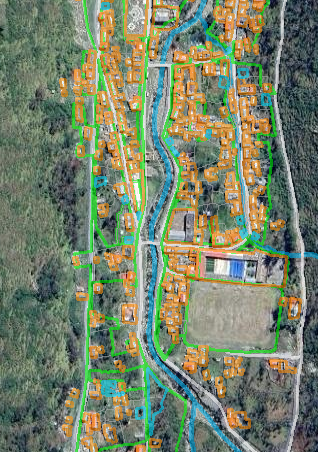
\includegraphics[width=0.85\textwidth,height=0.36\textheight,keepaspectratio]{figuras/05_zoom_sector_confluencia_estadio.png}
\caption{Sector de confluencia fluvial y área de expansión recreacional/deportiva.}
\label{fig:sector_confluencia}
\end{figure}

\subsection{Detalle Sector Sur: Complejo Recreacional, Piscina y SED-03}
La Figura~\ref{fig:sector_sur} presenta la zona sur del casco urbano, correspondiente al sector de la Piscina Municipal y salida hacia Crucero, servido por la Subestación SED-03 (Sur, 100 kVA) para 274 lotes:

\begin{figure}[H]
\centering
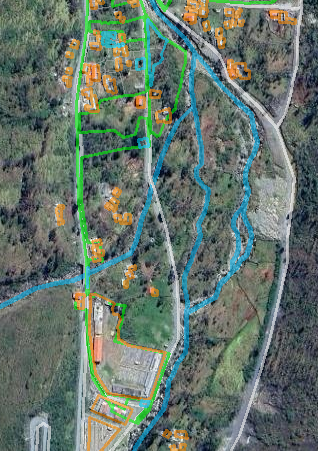
\includegraphics[width=0.85\textwidth,height=0.36\textheight,keepaspectratio]{figuras/06_zoom_sector_sur_piscina_salida.png}
\caption{Sector Sur: Complejo recreacional, piscina y cobertura de SED-03.}
\label{fig:sector_sur}
\end{figure}
